%% Requires compilation with XeLaTeX or LuaLaTeX
\documentclass[aspectratio=169,10pt,xcolor={table,dvipsnames},t]{beamer}
\usetheme{UCBerkeley}

\title[lecture 01]{Next Generation Data Centers and Energy Management Systems}
\subtitle{Lecture 1A: Class plan and rules}
\author{Prof. Thomas M. Schutzius}
\institute{Department of Mechanical Engineering}
\date{Fall 2026}

\begin{document}

\begin{frame}
  \titlepage
\end{frame}

% Uncomment these lines for an automatically generated outline.
%\begin{frame}{Outline}
%  \tableofcontents
%\end{frame}



{
\setbeamertemplate{background}{} % Hides background for this frame
\setbeamertemplate{footline}{}   % Reclaims the bottom space
\smallframetitle
	\begin{frame}
		\frametitle{Challenges and Opportunities in Data Centers}
		% Commands to include a figure:
		\begin{figure}
			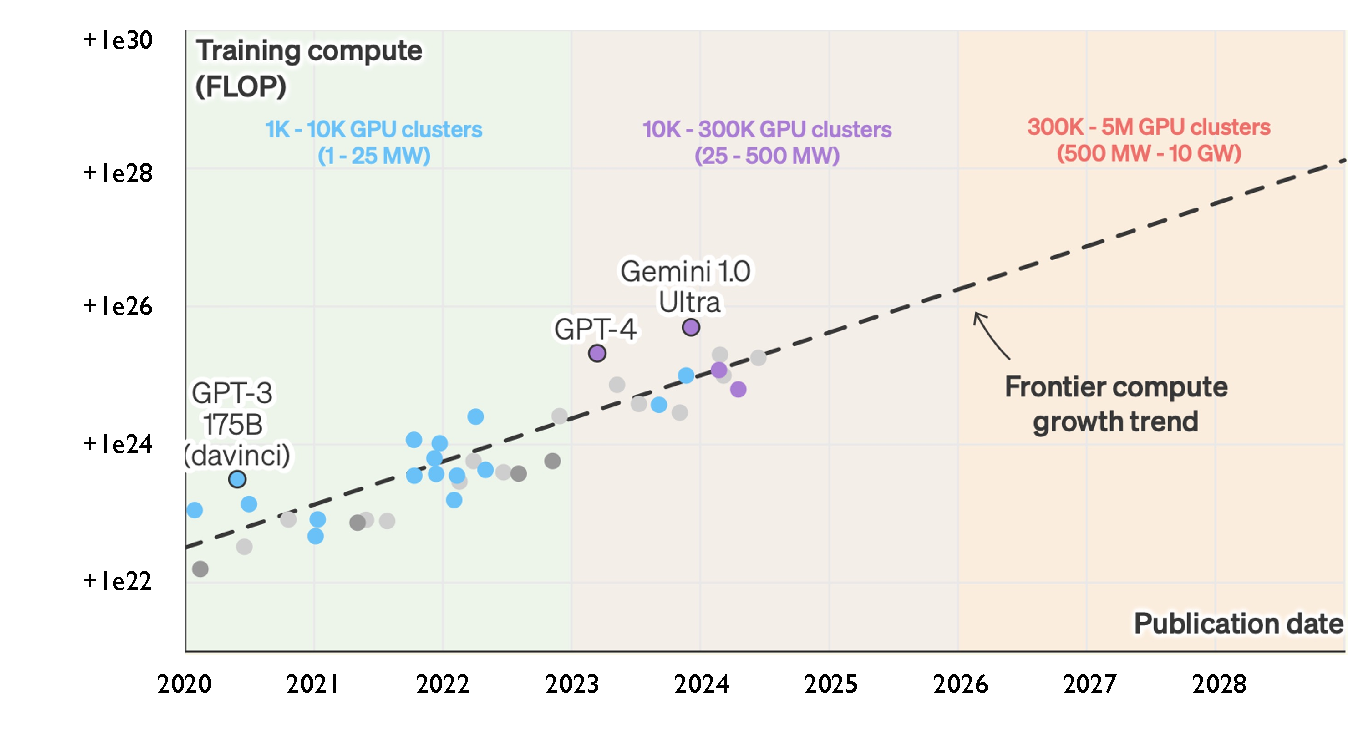
\includegraphics[width=0.8\textwidth]{figures/flops-llms.pdf}
			\vspace{-0.5cm}
		 \caption{\label{fig:flops-llms}``100k GPU clusters will seem normal in a few years'' -\href{https://www.youtube.com/watch?v=cu_3GMWl-rE}{R. Ober} (Chief Platform Architect), Nvidia}
		\end{figure}
	\end{frame}
}


{
\setbeamertemplate{background}{} % Hides background for this frame
\setbeamertemplate{footline}{}   % Reclaims the bottom space
\smallframetitle
	\begin{frame}
		\frametitle{Challenges and Opportunities in Data Centers}
		% Commands to include a figure:
		\begin{figure}
			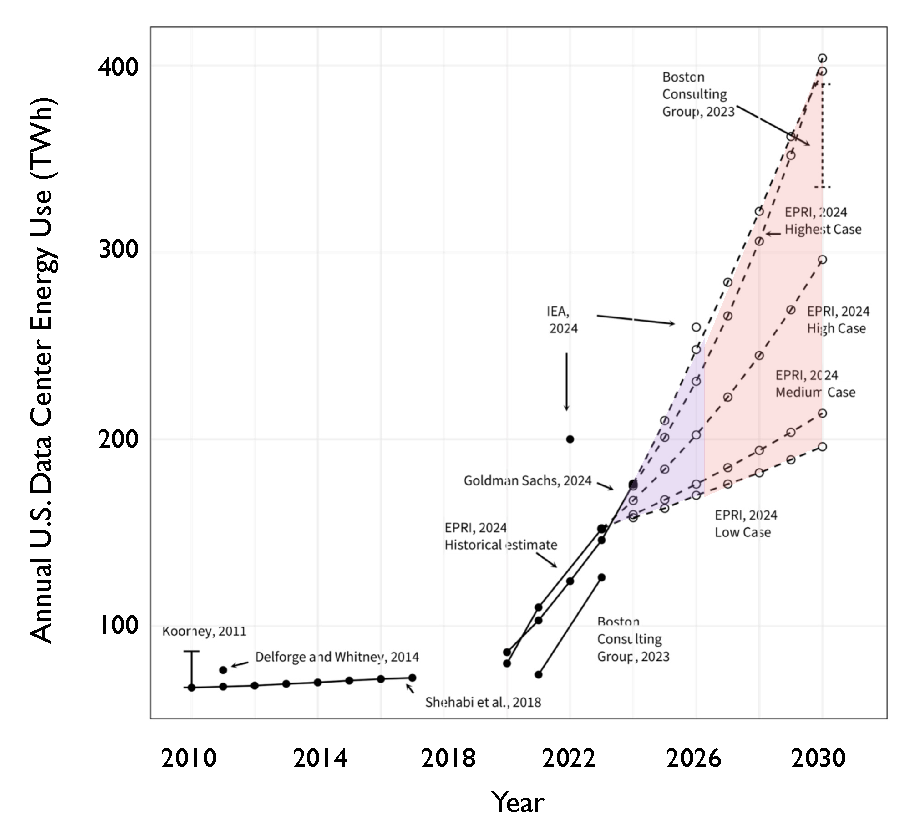
\includegraphics[width=0.5\textwidth]{figures/energy-use-data-centers-usa.pdf}
			\vspace{-0.5cm}
		\caption{\label{fig:energy-use-data-centers-usa}\href{https://eta-publications.lbl.gov/sites/default/files/2024-12/lbnl-2024-united-states-data-center-energy-usage-report.pdf}{eta-publications.lbl.gov}}
		\end{figure}
	\end{frame}
}


{
\setbeamertemplate{background}{} % Hides background for this frame
\setbeamertemplate{footline}{}   % Reclaims the bottom space
\smallframetitle
\begin{frame}
\frametitle{Teaching team}

\begin{columns}[T]

\begin{column}{0.48\textwidth}
\small
Ben Brown

		\begin{figure}
			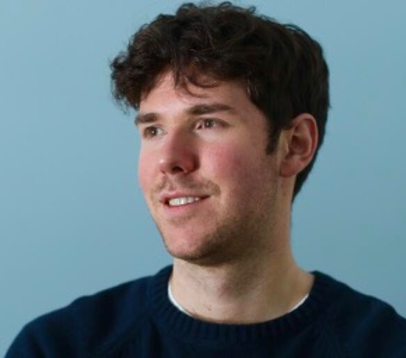
\includegraphics[width=0.5\textwidth]{figures/ben-brown.pdf}
			\vspace{-0.5cm}
%		\caption{\label{fig:ben-brown}\href{https://eta-publications.lbl.gov/sites/default/files/2024-12/lbnl-2024-united-states-data-center-energy-usage-report.pdf}{eta-publications.lbl.gov}}
		\end{figure}


\end{column}

\begin{column}{0.48\textwidth}
Amelia Stacey

		\begin{figure}
			
\includegraphics[width=0.5\textwidth]{figures/oski.jpeg}
			\vspace{-0.5cm}
%		\caption{\label{fig:ben-brown}\href{https://eta-publications.lbl.gov/sites/default/files/2024-12/lbnl-2024-united-states-data-center-energy-usage-report.pdf}{eta-publications.lbl.gov}}
		\end{figure}
\end{column}

\end{columns}
\end{frame}
}


{
\setbeamertemplate{background}{} % Hides background for this frame
\setbeamertemplate{footline}{}   % Reclaims the bottom space
\smallframetitle
	\begin{frame}
		\frametitle{Course Theme}
		% Commands to include a figure:
		\begin{figure}
			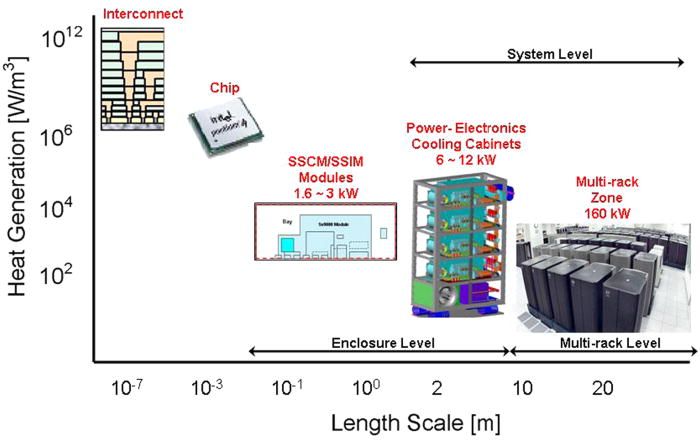
\includegraphics[width=0.65\textwidth]{figures/joshi2021reduced-figure-01.jpeg}
%			\vspace{-0.5cm}
		\caption{\label{fig:course-theme}J. Heat Transfer. 2012;134(3). doi:10.1115/1.4005150
}
		\end{figure}
	\end{frame}
}

{
\setbeamertemplate{background}{} % Hides background for this frame
\setbeamertemplate{footline}{}   % Reclaims the bottom space
\smallframetitle
	\begin{frame}
		\frametitle{Syllabus \& Learning Plan}
		% Commands to include a figure:
	\end{frame}
}

\end{document}
